\chapter{Teoretická část}\label{chap:teorie}

\section{Testování}

Testování je podstatnou součástí vývoje produktu a jeho softwaru. Cílem testování není pouze odhalení chyb v softwaru, ale také verifikace a validace softwaru. Validací softwaru kontrolujeme, zda software odpovídá specifikacím a je tím, co zákazník chtěl. Verifikací kontrolujeme správnost softwaru, tedy kontrolujeme, že systém ve vytvořených situacích se chová dle očekávání a specifikace. \cite{singh2012software}

Testování softwaru je zároveň dovednost. Při testování musí tester vybrat z nekonečného množství možných testů nějaký konečný počet, který nejlépe reprezentuje danou problematiku a pokrývá co největší možnou množinu všech možných případů. Zároveň musí vzít v potaz náročnost na vytvoření testu a na rigidnost vytvořeného testu proti změnám v softwaru. Tyto faktory poté ovlivňují i náklady na testování. \cite{fewster1999software}

Od testování softwaru lze také odvodit kvalitu softwaru. Kvalita softwaru se dá určit tím, jak moc vytvořený software odpovídá zadaným specifikacím~\cite{software_quality}. Tyto informace jsou poté velmi důležité pro managment. Díky nim může vyhodnocovat současný stav vývoje a upravovat plán na vývoj. 

Testování zároveň zvyšuje důvěru ve vyvíjený softwaru. Každý dobře navržený test snižuje šanci, že v softwaru existuje nepodchycená chyba. S každým rozsáhlým testováním se tato důvěra zvyšuje. \cite{fewster1999software}

\subsection{Rozdělení testů}

I když primární cíl testování je jednotný, přístupů k testování je několik. Vhodnost jednotlivých přístupů se mění na základě testované komponenty. Tyto přístupy se dají podle \cite{luo2001software} rozdělit do několika kategorií.

\subsubsection{Podle znalosti komponenty}

Testování se dá rozdělit podle přístupu k informacím, které o komponentách softwaru/systému víme. Tyto typy jsou:

\begin{description}
    \item[Black box testování] Nazýváno taktéž funkční testování. Na software se pohlíží jako na tzv. černou skříňku. O komponentě nebo celku nic nevíme a testujeme na základě funkcionálních požadavků, návrhu, specifikací nebo uživatelské dokumentace. 
    \item[White box testování] Se znalostí implementace testované části se snažíme vytvořit takové testy, které způsobí spouštění určitých částí testované komponenty. Cílem je co největší pokrytí testování dané komponenty.
    \item[Grey box testování] Kombinace Black box a White box testování. Při testování máme nějakou znalost implementace komponenty, ale je nižší, než při White box testování. \cite{khan2010different}
\end{description}

\subsubsection{Podle částí vývoje}

Testování podle částí vývoje se přibližuje vývojovému cyklu. Tyto kategorie jsou:  

\begin{description}
    \item[Testování jednotlivých částí] Více známé pod anglickým pojmem \uv{Unit testing}. Je to nejnižší úroveň testování. Testuje jednotlivé komponenty systému samostatně.
    \item[Integrační testování] Testování dvou a více komponent, které spolu vytváří nějaký větší celek softwaru. Často také využíván při testování částí, které nelze samostatně testovat.
    \item[Systémové testování] Testování softwaru jako celku. Testování se směřuje na testování funkčních požadavků. Zároveň je možno vyhodnocovat další požadavky na systém, jako spolehlivost, bezpečnost, atd.
    \item[Akceptační testování] U toho testování se systém dostane do rukou zákazníkovi/uživatelům. Cílem je otestování produktu u uživatelů softwaru a získání jejich zpětné vazby. 
\end{description}

Propojení testů a vývojového cyklu je dobře znázorněno na tzv. V-modelu, který můžeme vidět na obrázku \ref{fig:vmodel}. Na tomto modelu, nazývaném podle svého tvaru, můžeme vidět jednotlivé typy stádia vývoje a jejich korespondující ověřování v závislosti na čase.

\begin{figure}[htbp]
    \centering 
    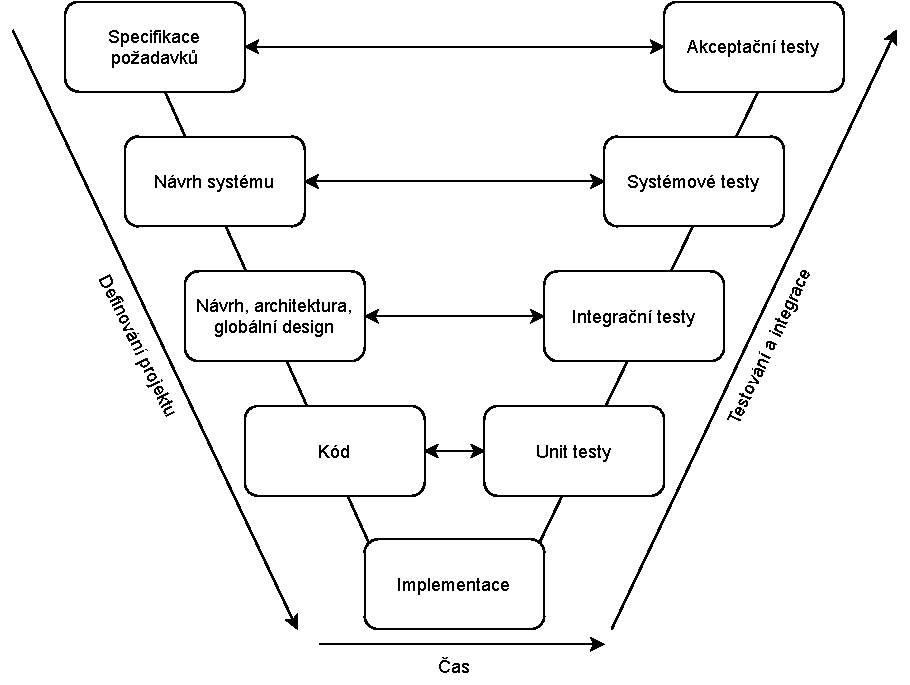
\includegraphics[width=0.9\textwidth]{assets/img/vmodel.pdf}
    \caption{V-model}
    \source{Vytvořeno dle předlohy z \cite{fewster1999software}}
    \label{fig:vmodel}
\end{figure}


\section{Automatizace testování}

Automatizace testování je odlišná od samotného testování. Automatizace testu neurčuje samotnou kvalitu testu. Pokud automatizujeme test, který nepřináší žádné nové benefity vývoji softwaru, tak poté dostaneme jeho výsledek pouze rychleji. \cite{fewster1999software} Proto tvorba testů je minimálně stejně důležitá, ne-li důležitější, jako samotná jejich automatizace. Automatizování je ale v mnoha ohledech v dnešní době standardem při testování, a to především díky jeho výhodám. Mezi tyto výhody podle \cite{fewster1999software} patří:

\begin{description}
    \item[Častější testování] S automatizací jsme schopni testovat software mnohem častěji, než při manuálním testování. Software může být testován například při každé jeho změně. Toto manuálně je velmi náročné, už jenom kvůli vysokému požadavku na lidské zdroje.  
    \item[Ulehčení testování] Test, který bude požadovat k jeho uskutečnění 200 uživatelů, není nemožný provést manuálně. S automatizací ale můžeme vstupy těchto uživatelů simulovat a tím celé testování zjednodušit.  
    \item[Lepší využití zdrojů] Tester je kvalifikovaný člověk a jeho využití na opakované vkládání vstupů a ověřování výstupů může být v některých případech plýtváním jeho časem.
    Taktéž při manuálním testování můžeme vyžadovat více účastníků testování, kteří všichni si musí vyhradit čas na testování. Díky automatizaci můžeme tyto zdroje využít víc efektivněji. Tester se například díky automatizaci může více soustředit na vytváření nových testů.
    \item[Konzistence] Při automatizaci testování každý běh testu proběhne naprosto identicky. Stejně jako ve vývoji, i v testování může dojít k lidské chybě. Díky automatizaci se šance lidské chyby snižuje. Toto zvyšuje konzistenci testování, než když se testy provádějí manuálně.
    \item[Snížení doby testování] Jednou automatizované testy mohou být provedeny mnohem rychleji a efektivněji, než při jejich manuálním spuštění. Toto způsobuje snížení potřebné doby na testování.
\end{description}

Automatizované testování následně může podporovat další procesy během vývoje. Mezi tyto procesy patří například proces kontinuální integrace nebo proces kontinuálního doručení softwaru. Proces kontinuální integrace se zaměřuje na integrování jednotlivých upravovaných částí do celkového softwaru. Oproti tomu proces kontinuálního doručení softwaru se zaměřuje na to, aby software vždy byl v takovém stavu, aby mohl být doručen zákazníkovi, nebo nasazen. \cite{ci_cd}

\section{Azure DevOps}

Azure DevOps server poskytuje vývojářům služby, které pomáhají při vývoji softwaru. Jeho cílem je podporovat jednotlivé procesy vývoje, což poté zrychluje vývoj softwaru. \cite{azure_devops} V této práci budu využívat několik služeb, které Azure DevOps server nabízí. Tyto služby budou:

\begin{description}
    \item[Azure Repos] Azure Repos je sada nástrojů, která umožňuje správu jednotlivých verzí softwaru. V této práci budeme používat systém správy verzí Git, který je Azure Repos podporovaný. \cite{azure_repos}
    \item[Azure Pipelines] Azure Pipelines umožňuje automaticky kompilovat a testovat vyvíjený software. Tím také podporuje procesy kontinuální integrace, kontinuálního nasazení softwaru nebo kontinuálního testování. \cite{azure_pipelines}
    \item[Azure Test Plans] Azure Test Plans přináší sadu nástrojů, které umožnují spravovat testování softwaru. Tyto nástroje umožňují správu testovacích sad a jednotlivých testů, ať už manuálních nebo automatizovaných. \cite{azure_test_plans}
    \item[Azure Artifacts] Azure Artifacts umožňuje publikování a verzování různých typů balíčků. Následně tato správa těchto balíčků může být využita při vydání těchto balíčků. Mezi podporované balíčky patří například NuGet, Maven nebo npm. Zároveň skrz Azure Artifact můžeme publikovat data z Azure Pipelines. \cite{azure_artifacts}
\end{description}

Azure DevOps server využívá při delegování úkolů tzv. agenty. Agent je výpočetní infrastruktura s nainstalovaným softwarem agenta, který pracuje na jedné určité úloze \cite{agent_docs}. Agent následně provádí například jednotlivé úkony definované v Azure Pipelines, jako kompilace, testování atd.

\section{Framework MSTest}

Framework MSTest je výchozí testovací framework, který je integrován do IDE Visual Studio. Díky tomu je také často nazýván jako \uv{Visual Studio Unit Testing Framework}. Framework započal jako nástroj spouštěný z příkazové řádky, který následně prováděl testování. Díky implementaci do Visual Studia je tento framework často preferován vývojáři, kteří používají Visual Studio pro vývoj. 

MSTest framework přináší nástroje, které jsou potřeba k verifikaci a validaci softwaru. V dnešní době framework MSTest V2 je open-source projekt, který je stále rozvíjen. Mezi jeho výhody patří podpora napříč platformami a rozšiřitelnost. \cite{mstest_descr}


\section{Průmyslová komunikace}\label{sec:fieldbus}

Při řešení průmyslové komunikace se často objevuje slovo \textit{fieldbus}. Běžný význam tohoto slova je \uv{Síť, která propojuje průmyslová zařízení jako kontrolery, PLC, regulátory atd.} \cite{fieldbus_thomesse}. Vznik těchto sítí je úzce spojený s historií vývoje informačních technologií. V době, kdy začali tyto sítě vznikat, nebyli dostupné komunikační technologie, jako dnes. Dostupné informační a telekomunikační sítě té doby nemohli uspokojit potřeby průmyslových sítí na deterministickou, spolehlivou a efektivní komunikaci \cite{future_of_ind_com}. 

V dobách vzniku těchto komunikačních protokolů bylo pro fyzické připojení využíváno různých protokolů -- například RS-485. Nedostatkem těchto protokolů avšak byli vysoké implementační náklady. S růstem popularity standardu IEEE 802.3 -- dnes často nazýván Ethernet -- se začalo zkoumat možné použití tohoto standardu při průmyslové komunikaci. Odborníci došli k závěru, že je možné při průmyslové komunikaci v reálném čase využít tento standard \cite{lee_ethernet_fieldbus}. V dnešní době je Ethernetový standard hojně využíván při přenosu průmyslové komunikace.


\subsection{Protokol Modbus}
Modbus je průmyslový komunikační protokol, který je umístěn na aplikační vrstvě ISO/OSI modelu. Tento protokol, vytvořený v roce 1979, umožňuje komunikaci typu klient-server mezi zařízeními na různých typech sítí a sběrnic. 

Protokol definuje strukturu zprávy (tzv. PDU -- Protocol Data Unit) nezávisle od komunikační vrstvy. Tato zpráva se avšak může rozšířit, v závislosti na způsobu přenosu této zprávy. V závislosti na typu sítě je poté tato zpráva rozšířena o další údaje. Tento celek se poté označuje jako ADU -- Application Data Unit. Tuto celou strukturu můžeme vidět znázorněnou na obrázku \ref{fig:modbus_frame}.~\cite{modbus}

\begin{figure}[htbp]
    \centering 
    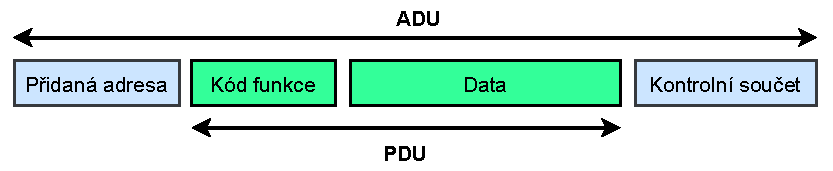
\includegraphics[width=\textwidth]{assets/img/modbusframe.pdf}
    \caption{Obecné znázornění jednoho rámce protokolu Modbus}
    \source{Vytvořeno dle předlohy z \cite{modbus}}
    \label{fig:modbus_frame}
\end{figure}

Podporované služby jsou definováno funkčními kódy, které jsou součástí požadavku. Kód funkce je uložen v jednom bajtu a tedy rozsah možných kódu je 1-255 (0 je nevalidní), kde rozsah 128-255 je rezervován pro chybové zprávy. Data zprávy poté slouží k upřesnění operace definované funkčním kódem. V určitých situacích muže postačovat v provedení operace funkční kód, data zprávy poté mají nulovou délku.

Modbus používá komunikaci požadavek-odpověď. Na požadavek klienta server odpovídá zprávou, kterou značí úspěch či neúspěch operace. V případě úspěchu server odesílá zpět zprávu se stejným funkčním kódem jako byl požadavek. V opačném případě odesílá zpět zprávu, která obsahuje stejný kód funkce jako byl kód funkce požadavku, ale tento kód má zároveň nastavený nejvýznamnější bit na 1. Zpráva v obou případech může poté obsahovat data, v závislosti na operacích. \cite{modbus}

V této práci se budu zaměřovat na použití protokolu ModbusTCP. Jak již z názvu vyplívá, ModbusTCP používá k přenosu zpráv protokol TCP/IP a Ethernet připojení. Zároveň používá stejnou komunikaci definovanou protokolem Modbus.

\subsection{Protokol EtherNet/IP}
Protokol EtherNet/IP (EtherNet/Industrial Protocol) je dalším dnes již široce používaným průmyslovým protokolem. Jak již z názvu vyplívá, protokol používá Ethernetový standard k propojení průmyslových zařízení. Ke komunikaci následně používá standardně používané protokoly TCP a UDP. Tento protokol byl poprvé představen v roce 2001 a od roku 2005 je standardizován. 

Protokol je umístěn na 5--7 vrstvě ISO/OSI modelu. V rámci sítě jsou jednotlivým uzlům přiřazeny předem definované profily. Profil reprezentuje typ zařízení se specifickými vlastnostmi. Profil zařízení a aplikační vrstva protokolu EtherNet/IP jsou vytvářeny protokolem CIP (Common Industrial Protocol). Tento protokol používá komunikaci na principu producent-konzument. Použitím společného protokolu CIP se následně dosahuje interoperability mezi všemi sítěmi, které ho podporují. 

Protokol CIP je objektově orientovaný. Každé zařízení je reprezentováno skupinou objektů. Každý z objektů obsahuje data, služby resp. příkazy a specifikaci funkcí. V rámci protokolu je poté definováno, jaké atributy musí každý objekt obsahovat.

Aplikační objekty obsahují data, které jsou specifická pro komunikující zařízeni. Výrobci mohou specifikovat i svoje vlastní objekty. Pro identifikaci dostupných objektů jsou sestaveny elektronické popisy zařízení, které obsahují potřebné informace ke konfiguraci zařízení v síti EtherNet/IP. 

Přenos v síti EtherNet/IP se odvíjí dle využitého protokolu pro přenos. Při použití protokolu TCP je přenos explicitní a je určen k přenosu typu žádost-odpověď mezi dvěma zařízeními. Naopak při použití protokolu UDP je přenos implicitní, který je pak určený pro cyklický přenos uživatelských a I/O dat. Komunikační model objektů CIP umožňuje lépe využít možnosti komunikačního kanálu. Přenos zprávy následně probíhá dle protokolu. Žadatel zahajuje komunikaci s cílovým zařízením odesláním žádosti k vytvoření komunikace, která obsahuje navrhované parametry spojení. Cílové zařízení následně odesílá potvrzení s přesnými parametry a navazuje spojení. Každé spojení je poté určeno identifikátorem. \cite{ethernet_ip}

\section{Testovaný produkt}

Hlavním cílem této práce je vytvoření testovací knihovny pro řadu zařízení SIMATIC ET 200, vyvíjený společností Siemens,~s.\,{}r.\,{}o, se zaměřením na zařízení SIMATIC ET 200SP. Řada produktů SIMATIC ET 200 přináší jednu z nejširších nabídek I/O zařízení. Produkty této řady můžeme vidět znázorněné na obrázku \ref{fig:et200}. Jak z obrázku můžeme vidět, každé zařízení obsahuje jiný stupeň ochrany v závislosti na jejich plánovaném umístěním. \cite{et200} 

\begin{figure}[htbp]
    \centering 
    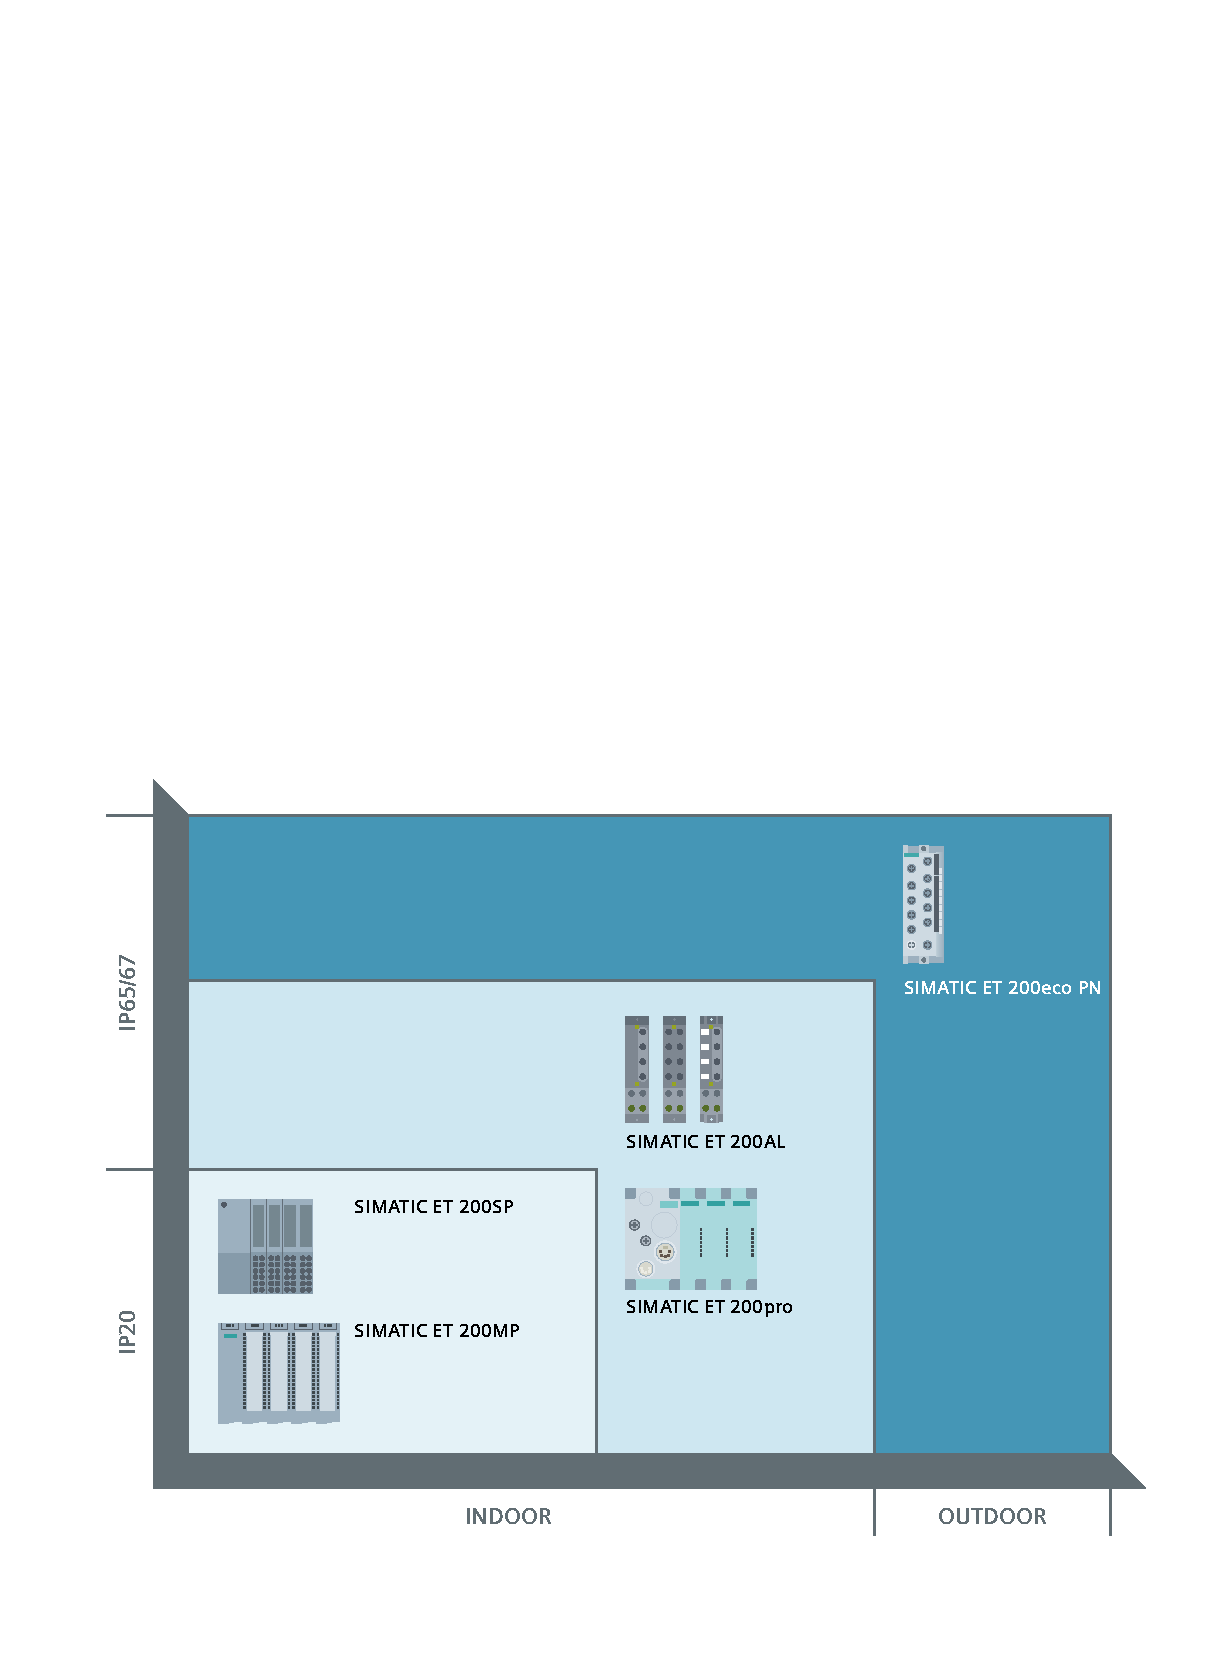
\includegraphics[width=0.87\textwidth]{assets/img/et200.pdf}
    \caption{Znázornění produktové řady SIMATIC ET 200}
    \source{Marketingové materiály firmy Siemens,~s.\,{}r.\,{}o \cite{et200}}
    \label{fig:et200}
\end{figure}

Zařízení SIMATIC ET 200SP, které můžeme vidět na obrázku \ref{fig:et200sp}, je určeno k umístění do kompaktních řídících kabinetů. Díky modulárnosti systému se systém může vysoce přizpůsobit potřebám jednotlivých průmyslů. Mezi tyto moduly patří standardní I/O moduly, komunikační moduly, technologické moduly nebo moduly ke startování motorů. Zároveň je velikou výhodou celkový kompaktní design. Jednotlivé moduly zároveň mohou být vyměňovány za běhu. \cite{et200sp}

SIMATIC ET 200SP využívá tzv. Multifieldbus technologii. Tato technologie umožňuje zařízení komunikovat na základě několika průmyslových protokolů. V rámci této práce se zaměříme na protokoly ModbusTCP a EtherNet/IP, které již byli dříve popsané.

\begin{figure}[htbp]
    \centering 
    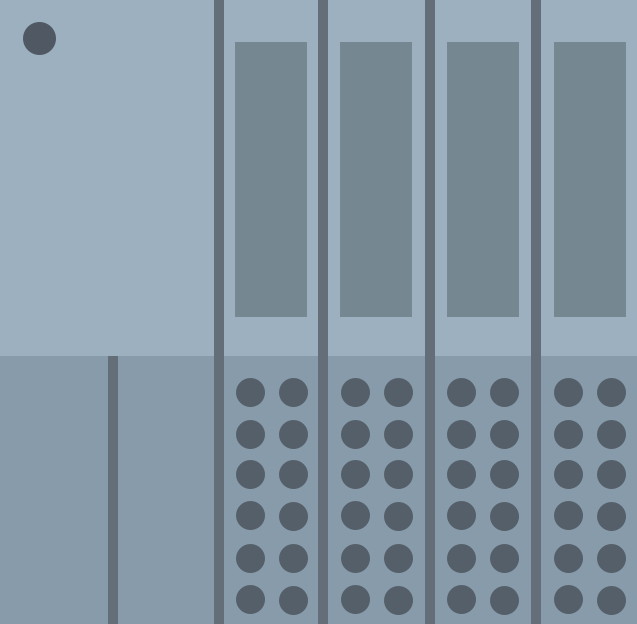
\includegraphics[width=\textwidth]{assets/img/et200sp.png}
    \caption{Zařízení SIMATIC ET 200SP}
    \source{Marketingové materiály firmy Siemens,~s.\,{}r.\,{}o \cite{et200sp}}
    \label{fig:et200sp}
\end{figure}